\documentclass[a4paper,12pt]{article}

\usepackage{cmap}
\usepackage[T2A]{fontenc}
\usepackage[utf8x]{inputenc}
\usepackage[english, russian]{babel}

\usepackage{misccorr} % в заголовках появляется точка, но при ссылке на них ее нет
\usepackage{amssymb,amsfonts,amsmath,amsthm}  
\usepackage{indentfirst}
\usepackage[usenames,dvipsnames]{color} 
\usepackage[unicode, colorlinks, urlcolor=magenta, linkcolor=black, pagecolor=black]{hyperref}
\usepackage{makecell,multirow} 
\usepackage{ulem}
\usepackage{graphicx}
\graphicspath{{img/}}
\usepackage{geometry}
\geometry{left=3cm,right=2cm,top=3cm,bottom=3cm,bindingoffset=0cm}
\usepackage{fancyhdr} 
\linespread{1.3} 
\frenchspacing 
\renewcommand{\labelenumii}{\theenumii)} 
\usepackage{caption}
%%%%%%%%%%%%%%%%%%%%%%%%%%%%%%%%%%%%%%%%%%%%%%%%%%%%%%%%%%%%%%%%%%%%%%%%%%%%%%%
%%%%%%%%%%%%%%%%%%%%%%%%%%%%%%%%%%%%%%%%%%%%%%%%%%%%%%%%%%%%%%%%%%%%%%%%%%%%%%%

\def\labauthor{Сарафанов Ф.Г.}
\def\labauthors{Сарафанов Ф.Г.}
\def\labnumber{22}
\def\labtheme{Определение коэффициента внутреннего трения (вязкости) жидкости}

%%%%%%%%%%%%%%%%%%%%%%%%%%%%%%%%%%%%%%%%%%%%%%%%%%%%%%%%%%%%%%%%%%%%%%%%%%%%%%%
%%%%%%%%%%%%%%%%%%%%%%%%%%%%%%%%%%%%%%%%%%%%%%%%%%%%%%%%%%%%%%%%%%%%%%%%%%%%%%%
	%применим колонтитул к стилю страницы
\pagestyle{fancy} 
	%очистим "шапку" страницы
\fancyhead{} 
	%слева сверху на четных и справа на нечетных
\fancyhead[LE,RO]{\labauthors} 
	%справа сверху на четных и слева на нечетных
\fancyhead[LO, RE]{Отчёт по лабораторной работе №\labnumber} 
	%очистим "подвал" страницы
\fancyfoot{} 
	% номер страницы в нижнем колинтуле в центре
\fancyfoot[CO,CE]{\thepage} 

%%%%%%%%%%%%%%%%%%%%%%%%%%%%%%%%%%%%%%%%%%%%%%%%%%%%%%%%%%%%%%%%%%%%%%%%%%%%%%% % колинтулы на страницах
%%%%%%%%%%%%%%%%%%%%%%%%%%%%%%%%%%%%%%%%%%%%%%%%%%%%%%%%%%%%%%%%%%%%%%%%%%%%%%%
\usepackage{float}
\usepackage[mode=buildnew]{standalone}
\usepackage{tikz} 

\usepackage{tikz,csvsimple}
\usetikzlibrary{scopes}
\usetikzlibrary{%
     decorations.pathreplacing,%
     decorations.pathmorphing,%
    patterns,%
    calc,%
    scopes,%
    arrows,%
    % arrows.spaced,%
}

\makeatletter
\newif\if@gather@prefix 
\preto\place@tag@gather{% 
  \if@gather@prefix\iftagsleft@ 
    \kern-\gdisplaywidth@ 
    \rlap{\gather@prefix}% 
    \kern\gdisplaywidth@ 
  \fi\fi 
} 
\appto\place@tag@gather{% 
  \if@gather@prefix\iftagsleft@\else 
    \kern-\displaywidth 
    \rlap{\gather@prefix}% 
    \kern\displaywidth 
  \fi\fi 
  \global\@gather@prefixfalse 
} 
\preto\place@tag{% 
  \if@gather@prefix\iftagsleft@ 
    \kern-\gdisplaywidth@ 
    \rlap{\gather@prefix}% 
    \kern\displaywidth@ 
  \fi\fi 
} 
\appto\place@tag{% 
  \if@gather@prefix\iftagsleft@\else 
    \kern-\displaywidth 
    \rlap{\gather@prefix}% 
    \kern\displaywidth 
  \fi\fi 
  \global\@gather@prefixfalse 
} 
\newcommand*{\beforetext}[1]{% 
  \ifmeasuring@\else
  \gdef\gather@prefix{#1}% 
  \global\@gather@prefixtrue 
  \fi
} 
\makeatother

\usepackage{booktabs}
\usepackage{pgfplots, pgfplotstable}

\pgfplotstableset{
    columns/mat/.style={%
    string type,
    column type=r,% 
    column name=\textsc{Материал}%
    },
    columns/d1/.style={column name=$d_1\text{, мм}$},
    columns/d2/.style={column name=$d_2\text{, мм}$},
    columns/d3/.style={column name=$d_3\text{, мм}$},
    columns/m/.style={column name=$m\text{, г}$},
    columns/dr/.style={column name=$\Delta{d}\text{, мм}$},
    columns/d/.style={column name=$<d>$},
    columns/r/.style={column name=$<r>$},
    empty cells with={--}, % replace empty cells with ’--’
    every head row/.style={before row=\toprule,after row=\midrule},
    every last row/.style={after row=\bottomrule}
  }
% \pgfplotstabletypeset[ % local config, applies only for this table
%     1000 sep={\,},
%     columns/info/.style={
%         fixed,fixed zerofill,precision=1,showpos,
%         column type=r,
%       }
%   ]

\begin{document}

\begin{titlepage}

\begin{center}

{\small\textsc{Нижегородский государственный университет имени Н.\,И. Лобачевского}}
\vskip 1pt \hrule \vskip 3pt
{\small\textsc{Радиофизический факультет}}

\vfill

{\Large Отчет по лабораторной работе №\labnumber\vskip 12pt\bfseries \labtheme}
	
\end{center}

\vfill
	
\begin{flushright}
	{Выполнил студент 410 группы\\ \labauthor\vskip 12pt Принял:\\ Менсов С.\,Н.}
\end{flushright}
	
\vfill
	
\begin{center}
	Нижний Новгород, 2016
\end{center}

\end{titlepage}



\tableofcontents
\newpage

\section*{Введение} % (fold)
\label{sec:input}

\textbf{Вязкостью} или внутренним трением называется явление возникновения силы трения между слоями текущей 
жидкости или газа, параллельными направлению течения. 

При течении жидкости слой, прилегающий к стенке цилиндра с жидкостью прилипает так, что его скорость становится равна нулю. Следующий слой движется, но из-за хаотичного перемещения молекул некоторые из них попадают в первый слой, теряя импульс при столкновении. 

Третий слой передает импульс второму и т.д. В результате этого наибольшей скоростью обладает та часть жидкости, которая более всего удалена от  стенки -- радиальная ось сосуда, а скорости всех остальных слоев уменьшаются по мере приближения к стенке.

При ламинарном течении жидкости скорость в цилиндре зависит от радиуса по квадратичному закону (распределение по параболе):
\begin{equation}
	v(r)=v_0(1- \frac{r^2}{R^2}),
\end{equation}

где $r$ -- расстояние от радиальной оси, $R$ -- радиус сосуда, $v_0$ -- максимальная скорость в потоке жидкости.

Так как изменение импульса в единицу времени равно силе, то это и приводит к появлению силы внутреннего трения. Такая сила трения может описываться \textbf{законом вязкости Ньютона}:
\begin{equation}
	F = - \eta \frac{\partial v}{\partial n}S,
\end{equation}

Вязкости жидкостей значительно отличаются от вязкостей газов, много больше по величине и резко уменьшаются с повышением 
температуры (тогда как для газов увеличиваются). 

Целью настоящей работы является определение  коэффициента вязкости разведенного глицерина одним из методов -- методом Стокса.

Стокс вывел формулу для силы сопротивления $F_\text{тр}$,  действующей на твёрдый шар при его медленном равномерном движении в неограниченной вязкой жидкости. Эта формула имеет вид:
\begin{equation}
	F_\text{тр} = 6{\pi}r{\eta}v
\end{equation}

где $r$ и $v$ -- радиус и скорость шара, $\eta$— динамический коэффициент вязкости жидкости.

% section введение (end)


\section{Оборудование} % (fold)
\label{sec:the}

% section теория_эксперимента (end)

\begin{figure}[H]
	\centering
\begin{tikzpicture}[
    force/.style={>=latex,draw=blue,fill=blue, very thick},
    axis/.style={densely dashed,black!60,font=\small},
    interface/.style={draw=gray!60,
        postaction={draw=gray!60,decorate,decoration={border,angle=-135,
                    amplitude=0.3cm,segment length=2mm}}},
]
	\def\w{40mm}
	\def\h{90mm}
	\draw[interface] (-10mm,0) -- (\w+10mm,0);

	\draw  (0,\h) -- (0,0) -- (\w,0) -- (\w,\h);

	\foreach \c in {0,10,...,70}{
 		\draw (10 mm, 80 mm - \c mm) node[left, xshift=-10mm] {\c};
 		\draw (0.3,80 mm - \c mm) -- (0.7,80 mm - \c mm);
	}

 	\foreach \d in {10,11,...,80}{
 		\draw (0.4,\d mm) -- (0.6,\d mm);
 	}

	\draw [axis, ->] (\w+10mm,\h-10mm) --(\w+10mm,10mm) node [below] {$+x$};

	\coordinate (C) at (\w/2, 60mm);
	\draw [fill=black!30] (C) circle (2.5mm);

	\draw[force, ->] (C) -- ++ (0, 10mm) node [right] {$\vec{F}_\text{арх}$};
	\draw[force, ->] (C) -- ++ (0, 20mm) node [right] {$\vec{F}_\text{тр}$};

	\draw[force, ->] (C) -- ++ (0,  -20mm) node [right] {$m\vec{g}$};

	\draw [fill=black] (C) circle (0.5mm);

	\draw [<->] (0,5mm) --(\w,5mm) node [above, pos=0.5] {$2R$};

	\draw[axis] ($(C)+(0,2.5mm)$) --($(C)+(10mm,2.5mm)$);
	\draw[axis] ($(C)+(0,-2.5mm)$) --($(C)+(10mm,-2.5mm)$);

	\draw[<->] ($(C)+(10mm,2.5mm)$)--($(C)+(10mm,-2.5mm)$) node [right, pos=0.5] {$2r$};

	\draw [fill=black, opacity=0.1] (0,0) -- (0,\h-8mm) -- (\w,\h-8mm) -- (\w,0) -- cycle;

\end{tikzpicture}	
	\caption{Рисунок установки к задаче о движении в вязкой жидкости}
	\label{fig:cxem}
\end{figure}

Для проведения опытов используется стеклянный цилиндрический сосуд радиусом $R=4.63$ см со шкалой (рис. \ref{fig:cxem}).

В сосуде находится глицерин с замеренной плотностью -- $1.22$ г/см$^3$.  

В глицерин на небольшом погружении (порядка 1--2 см) до 0 на шкале погружается, удерживаемый пинцетом, шарик. 

Шарик отпускается без начальной скорости по центру сосуда, чтобы минимизировать влияние стенок сосуда.

В эксперименте использовались стальной и пластмассовый шарики, замеренные микрометром.

\begin{table}[H]
	\caption{Размеры шариков}
	\label{tab:sphere}
	\centering
	\pgfplotstableread[col sep = comma]{experience/st.csv}{\loadedtable}
	\pgfplotstabletypeset{\loadedtable}
\end{table}


Незадолго до освобождения шарика включается видеокамера с минимальной частотой съемки $\omega=20$ Гц, движимая примерно параллельно шарику.

% На время, соответствующее началу первого опыта, в лабораторном помещении была температура $24\ C^\circ$, последнего опыта -- $25\ C^\circ$.

% \vspace{1em}
  % $\Delta{t}=0.06$ с, $\Delta{R}=0.05$ мм, $\Delta{d}=0.01$ мм, $\rho_\text{пластм}=(2.00\pm0.03)$ $\frac{\text{г}}{\text{см}^3}$

\section{Движение шарика в бесконечной вязкой среде} % (fold)
\label{sec:eq}

% section движение_шарика_в_бесконечной_вязкой_среде (end)

При движении на шарик действуют три силы: сила внутреннего трения $\vec{F}_\text{тр}$, сила тяжести $m\vec{g}$ и сила  Архимеда $\vec{F}_\text{арх}$ (рис. \ref{fig:cxem}).

\def\rhos{\rho_\text{шар}}
\def\rhoz{\rho_\text{жид}}
\def\Q{g\frac{\rhos-\rhoz}{\rhos}}
	\def\K{\frac{2}{9}gr^2\frac{\rhos-\rhoz}{\eta}}
\def\C{\Q-kv}%
\begin{gather}
	\beforetext{Запишем II закон Ньютона} m\vec{a}=\vec{F}_\text{тр}+m\vec{g}+\vec{F}_\text{арх}\\
	\beforetext{Где сила Стокса} F_\text{тр}=6\pi\eta{r}v\\
	\label{eq:ox}\beforetext{В проекции на $x$:}ma=mg-6\pi\eta{r}v-\rhoz{}gV\\
	\beforetext{}V=\frac{4}{3}\pi{r^3}, m=\rhos{}V\\
	\beforetext{Перепишем (\ref{eq:ox}):}ma=mg-6\pi\eta{r}v-\rhoz{}gV
\end{gather}
\begin{gather}
	\beforetext{Введем константу $k$:}k=6\pi\eta{r}\cdot \frac{1}{V\rhos}=\frac{6\pi\eta{r}}{m}\\
	\rhos{V}\frac{dv}{dt}=gV(\rhos-\rhoz)-kv \cdot V{\rhos}\\
	\frac{dv}{\C}=dt\\
	\beforetext{Замена переменной:   } \ \ c=\C\\
	dc=-k\,dv
	%\\
\end{gather}
\begin{gather}	
	-\frac{1}{k}\int^{\Q-kv(t)}_{\Q-kv_0} \frac{dc}{c} = \int_{0}^{t} dt\\
	\ln\left(\frac{\Q-kv(t)}{\Q-kv_0}\right)=-kt\\
	\frac{\Q-kv(t)}{\Q-kv_0}=e^{-kt}\\
	{\Q-kv(t)}=e^{-kt}({\Q-kv_0})\\
	kv(t)=e^{-kt}kv_0-e^{-kt}\Q+\Q
\end{gather}
\begin{gather}	
	kv(t)=\Q(1-e^{-kt})+e^{-kt}kv_0\\
	v(t)=\Q\frac{1-e^{-kt}}{k}+e^{-kt}v_0\\
	v(t)=Vg\frac{\rhos-\rhoz}{6\pi\eta{r}}({1-e^{-kt}})+e^{-kt}v_0
\end{gather}
\begin{gather}
	v(t)=\frac{2}{9}gr^2\frac{\rhos-\rhoz}{\eta}\cdot({1-e^{-kt}})+e^{-kt}v_0, \text{ где } k=\frac{6\pi\eta{r}}{m}.\\%
	s(t)=\int_0^{s(t)}v(t)\ dt = \K\cdot (\frac{e^{-kt}}{k}+t)-\frac{e^{-kt}v_0}{k}
\end{gather}
% \begin{gather}

\subsection{Путь установления и установившаяся скорость}
    
Для движения без начальной скорости
\begin{gather}
	v(t)=\frac{2}{9}gr^2\frac{\rhos-\rhoz}{\eta}\cdot({1-e^{-kt}})\\
	s(t)=\K\cdot (\frac{e^{-kt}}{k}+t)
\end{gather}
\begin{gather}
	1-e^{-kt^*}=\alpha=0.95\\
	e^{-kt^*}=\beta=0.05\\
	-kt^*=\ln{\beta}\\
	t^*=-\frac{1}{k}\ln{\beta}=-\frac{m}{6\pi\eta{r}}\ln{\beta}\\
	s^*=\K\cdot(\frac{\beta-\ln{\beta}}{k})=%
	\frac{m}{27\pi}gr\frac{\rhos-\rhoz}{\eta^2}(\beta-\ln{\beta})
\end{gather}

$t^*$ -- время установления, когда скорость будет отличаться от установившейся $v_\text{уст}$ на бесконечности не более чем в $\alpha$ раз.

$s^*$ -- соответственно путь установления, когда скорость отличается от установившейся $v_\text{уст}$ на бесконечности не более чем в $\alpha$ раз.

\begin{gather}
	\label{eq:v_ust}
	v_\text{уст}=\lim_{t \to \infty}{\left[\K\cdot(1-e^{-kt})\right]}=\K
\end{gather}

\section{Влияние стенок сосуда}

Условие бесконечной среды, заложенное в решении силы Стокса,  не может быть соблюдено экспериментально, и попытки проверки формулы Стокса обнаружили заметное влияние стенок сосуда. 

Частный случай движения в конечном цилиндре был рассмотрен Ладенбургом, который вывел поправки на влияние радиуса  $R$ и высоты $H$ цилиндра:
\begin{equation}
	F=F_\text{стокса}\cdot(1+2.4\frac{r}{R})\cdot(1+3.3\frac{r}{H})
\end{equation}

Нетрудно показать существование такой поправки.

Рассмотрим случай, когда жидкость бесконечна. Имеем невозмущенное решение Стокса
\begin{equation}
	\label{eq:st}
	F=6\pi\eta{r}v
\end{equation}

Будем постепенно уменьшать радиус сосуда. Ясно, что при его уменьшении будет оказывать влияние явление прилипания крайних слоев жидкости к стенкам сосуда -- тормозящая сила увеличится. 

Ясно, что в пределах размеров, много больших размеров молекул жидкости, безразлично, какое действие совершать: увеличивать радиус сосуда или во столько же уменьшать радиус шарика. Эти действия подобны.

Тогда введем коэффициент $p=\frac{r}{R}$ -- малый параметр.

Новую силу можно записать в виде 
\begin{equation}
	F=6\pi\eta{r}v\cdot\alpha,
\end{equation}

где $\alpha$ зависит от малого параметра $p$ и при параметре, стремящемся к 0, стремится к невозмущенному решению (\ref{eq:st}).

Тогда можем разложить $\alpha(p)$ в ряд Тейлора по малому параметру:
\begin{equation}
	\alpha(p)=1+Ap+Bp^2+\ldots
\end{equation}

Так как $p$ мало, можем пренебречь высшими степенями. Тогда поправка примет вид
\begin{equation}
	F=6\pi\eta{r}v\cdot(1+A\frac{r}{R})
\end{equation}

Ясно, что аналогичные рассуждения возможны для малого параметра $\frac{r}{H}$. Тогда сила Стокса примет вид:

\begin{equation}
	F=F_\text{стокса}\cdot(1+A\frac{r}{R})\cdot(1+B\frac{r}{H})
\end{equation}

\section{Экспериментальные данные}

\begin{table}[H]
	\centering

	% \caption{Caption for image}	
	\foreach \x in {1,2,3}{
		\begin{minipage}[c]{0.32\textwidth}
			\centering

		    % \label{fig:sample_figure}		
			\pgfplotstableread[col sep = comma]{experience/pl\x.csv}{\loadedtable}
			\pgfplotstabletypeset[
		    columns/s/.style={column name=$S\text{, см}$},
		    columns/t/.style={column name=$t\text{, с}$},
		    columns/v/.style={column name=$v\text{, см/с}$},
		    empty cells with={--}, % replace empty cells with ’--’
		    every head row/.style={before row=\toprule,after row=\midrule},
		    every last row/.style={after row=\bottomrule},
		    1000 sep={\,},
		    columns/info/.style={
		        fixed,fixed zerofill,precision=1,showpos,
		        column type=r,
		      }
		     ]{\loadedtable}
		\end{minipage}	
 	}
	\caption{Пластмассовые шарики}
	 \label{tab:sphere_pl}
\end{table}
\begin{figure}[H]
		\begin{minipage}[c]{0.49\textwidth}
			% \centering
			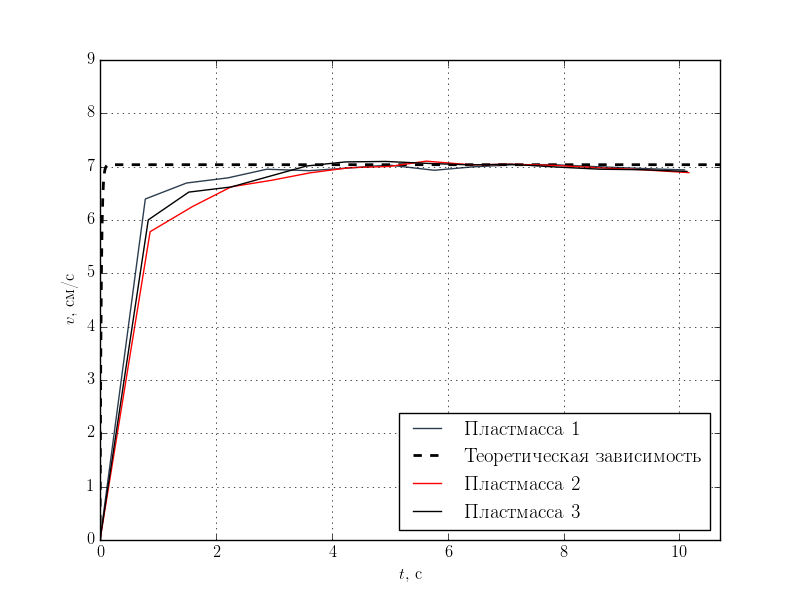
\includegraphics[width=1\textwidth]{img/plastic123.png}
			% \caption{Caption here}			
		\end{minipage}	
		\begin{minipage}[c]{0.49\textwidth}
			\centering
			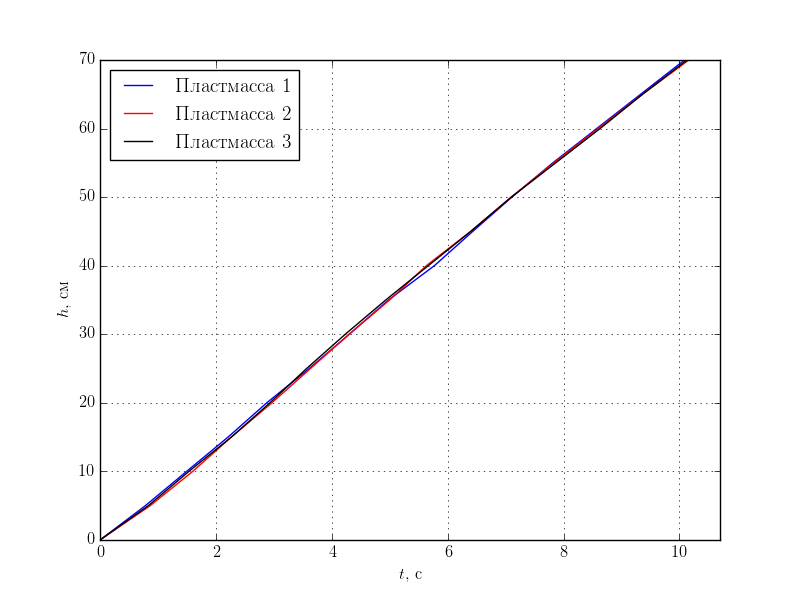
\includegraphics[width=1\textwidth]{img/plastic123-s.png}
			% \caption{Caption here}			
		\end{minipage}		
	\caption{Зависимости пути от времени и скорости от времени для пластмассовых шариков (эскизы)}
	\label{fig:figure1}
\end{figure}

\begin{table}[H]

	\centering
	% \caption{Caption for image}	
	\foreach \x in {1,2,3}{
		\begin{minipage}[c]{0.32\textwidth}
			\centering

		    % \label{fig:sample_figure}		
			\pgfplotstableread[col sep = comma]{experience/st\x.csv}{\loadedtable}
			\pgfplotstabletypeset[
		    columns/s/.style={column name=$S\text{, см}$},
		    columns/t/.style={column name=$t\text{, с}$},
		    columns/v/.style={column name=$v\text{, см/с}$},
		    empty cells with={--}, % replace empty cells with ’--’
		    every head row/.style={before row=\toprule,after row=\midrule},
		    every last row/.style={after row=\bottomrule},
		    1000 sep={\,},
		    columns/info/.style={
		        fixed,fixed zerofill,precision=1,showpos,
		        column type=r,
		      }
		     ]{\loadedtable}
		\end{minipage}	
 	}
	\caption{Стальные шарики} 	
	\label{tab:sphere_st}	
\end{table}
\begin{figure}[H]
		\begin{minipage}[c]{0.49\textwidth}
			% \centering
			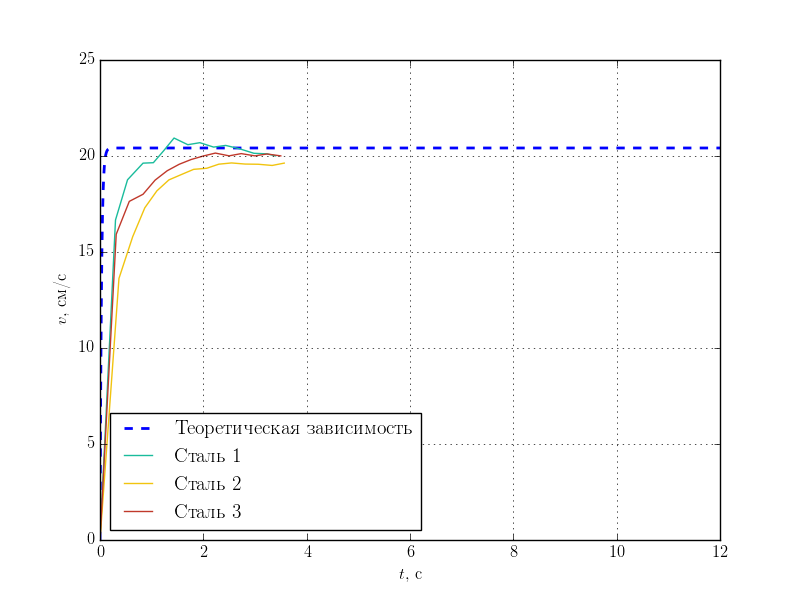
\includegraphics[width=1\textwidth]{img/steel123.png}
			% \caption{Caption here}			
		\end{minipage}	
		\begin{minipage}[c]{0.49\textwidth}
			\centering
			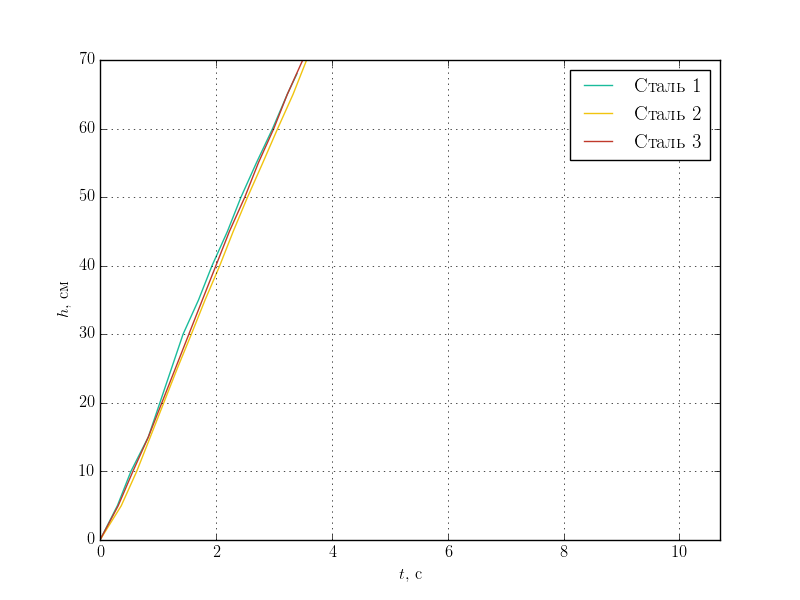
\includegraphics[width=1\textwidth]{img/steel123-s.png}
			% \caption{Caption here}			
		\end{minipage}		
	\caption{Зависимости пути от времени и скорости от времени для стальных шариков (эскизы)}
	\label{fig:figure1}
\end{figure}

\begin{table}[H]
	% \label{tab:sphere_st}
	\centering
		\begin{minipage}[c]{0.49\textwidth}
			\centering

		    % \label{fig:sample_figure}		
			\pgfplotstableread[col sep = comma]{experience/st5.csv}{\loadedtable}
			\pgfplotstabletypeset[
		    columns/s/.style={column name=$S\text{, см}$},
		    columns/t/.style={column name=$t\text{, с}$},
		    columns/v/.style={column name=$v\text{, см/с}$},
		    empty cells with={--}, % replace empty cells with ’--’
		    every head row/.style={before row=\toprule,after row=\midrule},
		    every last row/.style={after row=\bottomrule},
		    1000 sep={\,},
		    columns/info/.style={
		        fixed,fixed zerofill,precision=1,showpos,
		        column type=r,
		      }
		     ]{\loadedtable}
		\end{minipage}	
		\begin{minipage}[c]{0.49\textwidth}
			\centering

		    % \label{fig:sample_figure}		
			\pgfplotstableread[col sep = comma]{experience/pl6.csv}{\loadedtable}
			\pgfplotstabletypeset[
		    columns/s/.style={column name=$S\text{, см}$},
		    columns/t/.style={column name=$t\text{, с}$},
		    columns/v/.style={column name=$v\text{, см/с}$},
		    empty cells with={--}, % replace empty cells with ’--’
		    every head row/.style={before row=\toprule,after row=\midrule},
		    every last row/.style={after row=\bottomrule},
		    1000 sep={\,},
		    columns/info/.style={
		        fixed,fixed zerofill,precision=1,showpos,
		        column type=r,
		      }
		     ]{\loadedtable}
		\end{minipage}			
 	% }
	\caption{Подробное исследование нескольких бросков}	 	
\end{table}

\newpage
\section{Вязкость глицерина} % (fold)

\begin{equation}
	s^*=\frac{m}{27\pi}gr\frac{\rhos-\rhoz}{\eta^2}(\beta-\ln{\beta})	
\end{equation}

Для пластмассы путь установления до скорости, отличающейся не более чем на $5\%$ от установившейся, составляет $0.44\pm0.2$ cм, для стали --- $1.92\pm0.27$ см. 

Взяв участок пути, на котором координата больше пути установления, но достаточно далека от дна, получим значение скорости, близкой к установившейся, и  сможем рассчитать значение вязкости глицерина  из формулы (\ref{eq:v_ust}):
\begin{equation}
	{\eta}=\frac{2}{9}gr^2\frac{\rhos-\rhoz}{v_\text{уст}\cdot(1+2.4\frac{r}{R})}
\end{equation}

Рассчитаем относительную погрешность определения вязкости:
\begin{gather}
	\varepsilon{(\eta)}=\frac{2\Delta{\rho}}{\rhos-\rhoz}+\varepsilon(v)+\frac{3\Delta{r}}{r}\\
	\varepsilon{(v)}=\frac{\Delta{x}}{x}+\frac{\Delta{t}}{t}
	%\frac{2}{9}gr^2\frac{\rhos-\rhoz}{v_\text{уст}\cdot(1+2.4\frac{r}{R})}
\end{gather}
% section вязкость_глицерина (end)

Для данных по пластмассовым шарикам (табл. \ref{tab:sphere_pl}) получили значения вязкости $2.12\pm9.1\%$ Пз, $2.19\pm8.8\%$ Пз, $2.11\pm8.92\%$ Пз.

Для данных по стальных шарикам (табл. \ref{tab:sphere_st}) получили значения вязкости $2.52\pm11.9\%$ Пз, $2.57\pm12.3\%$ Пз, $2.55\pm12.1\%$ Пз.

\begin{figure}[H]
	\captionsetup[figure]{skip=-1em}	
	\centering
	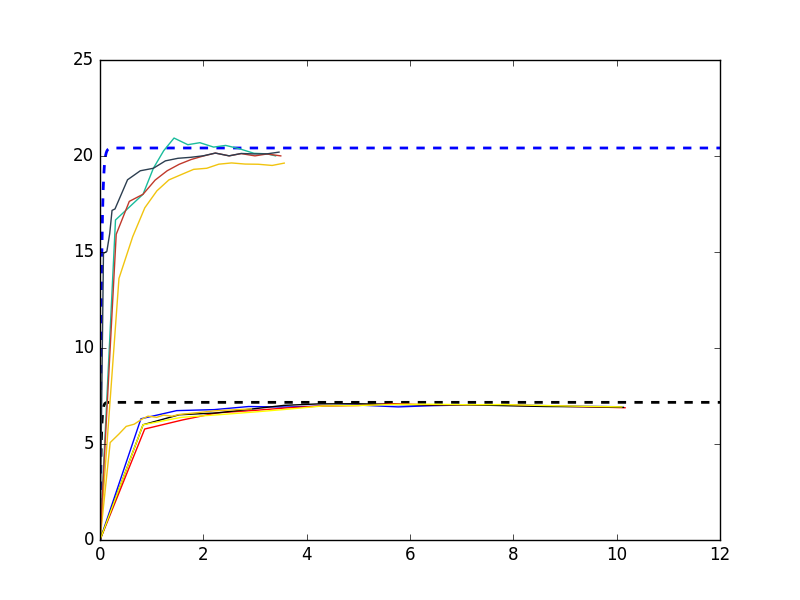
\includegraphics[width=0.8\textwidth]{img/two.png}
	\caption{Сводный график скоростей шариков и теоретических зависимостей (эскиз)}
	\label{fig:summary}
\end{figure}

\def\plastic{\def\Xstep{5/4}\def\XIo{1}\def\XIIo{2}\def\XNo{10}%
\includestandalone{tikz/plotter_.tex}}

\def\steel{\includestandalone{tikz/plotter_.tex}}

\def\includecsv[#1]#2{\def\file{#1}#2}
	

\subsection{Зависимость пути от времени}
\captionsetup[figure]{skip=-1em}	

\foreach \i in {1,2,3} {
	\begin{figure}[H]
		\includecsv[../experience/pl\i.csv]{\plastic}
		\caption{Пластмасса - опыт \i}
	\end{figure}
}

\foreach \i in {1,2,3} {
	\begin{figure}[H]
		\includecsv[../experience/st\i.csv]{\steel}
		\if\i5%
			\caption{Сталь - опыт 4}
		\else%
			\caption{Сталь - опыт \i}
		\fi		
	\end{figure}
}


% \begin{figure}[H]
% 	\def\yvar{v}
% 	\def\Yi{3}\def\Yii{6}\def\Yn{21}\def\Ystep{1/3}
% 	\def\ylabel{$v$, см/c}
% 	\includecsv[../experience/st1.csv]{\steel}	
% \end{figure}

\subsection{Зависимость скорости от пути}
\captionsetup[figure]{skip=-1em}	

\foreach \i in {1,2,3} {
	\begin{figure}[H]
		\def\yvar{v}
		\def\xvar{s}
		\def\Xerr{1}
		\def\Yerr{1}
		\def\Yi{3}\def\Yii{6}\def\Yn{21}\def\Ystep{1/3}
		\def\Xstep{1/5}\def\XIo{10}\def\XIIo{20}\def\XNo{70}
		\def\ylabel{$v$, см/c}
		\def\xlabel{$S$, см}
		\includecsv[../experience/pl\i.csv]{\steel}	
		\caption{Пластмасса - опыт \i}
	\end{figure}	
}


\foreach \i in {1,2,3} {
	\begin{figure}[H]
		\def\yvar{v}
		\def\xvar{s}
		\def\Xerr{1}
		\def\Yerr{1}
		\def\Yi{3}\def\Yii{6}\def\Yn{21}\def\Ystep{1/3}
		\def\Xstep{1/5}\def\XIo{10}\def\XIIo{20}\def\XNo{70}
		\def\ylabel{$v$, см/c}
		\def\xlabel{$S$, см}
		\includecsv[../experience/st\i.csv]{\steel}	
		\caption{Сталь - опыт \i}
	\end{figure}	
}

\newpage
\section*{Заключение}
\addcontentsline{toc}{section}{Заключение}

Замерили массы шариков -- $0.24$ и $0.265$ грамм, плотность пластмассы -- $2.2$ г/см$^3$, радиусы шариков -- $2\pm0.02 mm$, $5.92\pm0.02 mm$.

Сняли зависимости координат шарика по радиальной оси во времени для набора опытов. 

Методом раскадровки преобразовали видеоряд опыта в таблицу координат и скоростей по времени.

Проанализировав данные, нашли установившуюся скорость пластмассового шарика -- $7\pm4\%$ см/с, стального шарика -- $20\pm11\%$ см/с.

Для данных по пластмассовым шарикам (табл. \ref{tab:sphere_pl}) получили значения вязкости $2.12\pm9.1\%$ Пз, $2.19\pm8.8\%$ Пз, $2.11\pm8.92\%$ Пз.

Для данных по стальных шарикам (табл. \ref{tab:sphere_st}) получили значения вязкости $2.52\pm11.9\%$ Пз, $2.57\pm12.3\%$ Пз, $2.55\pm12.1\%$ Пз.

Вывели зависимости скорости, координат по времени для шарика, движушегося в бесконечной вязкой среде.

Построили графики зависимостей для всех опытов, эскизы для сводных графиков.

Изучили влияние вязкого трения на характер движения сферического тела в цилиндрическом сосуде.

Нашли число Рейнольдса для данного эксперимента
\begin{equation}
	\mathrm{Re}=\frac{\rho vD}{\eta}=48.3,
\end{equation}
где $v$ -- характерная скорость -- $0.2$ м/с, $\rho$ -- плотность глицерина -- $1220$ кг/м$^3$ $D$ -- характерный размер -- $0.0926$ м, $\eta$ -- средняя вязкость -- $0.23$ Па$\cdot$с.

Характер движения -- ламинарный.

Объяснили существование поправок Ладенбурга влияния стенок и дна цилиндрического сосуда на силу внутреннего трения.


\newpage
\subsection*{Ответы на вопросы}
\addcontentsline{toc}{subsection}{Ответы на вопросы}


\end{document}
